
\section{Equations to Define Velocity and Acceleration\footnote{
1990-93 Dept. of Physics and Astronomy, Dickinson College. Supported by FIPSE
(U.S. Dept. of Ed.) and NSF. Portions of this material may have been modified
locally and may not have been classroom tested at Dickinson College.
}}

\makelabheader %(Space for student name, etc., defined in master.tex or labmanual_formatting_commands.tex)

\textbf{Objectives} 

To learn how physicists use mathematical equations to describe simple one-dimensional
motions by:

\begin{enumerate}
\item Understanding the mathematical definitions of both average and instantaneous
velocity and acceleration as well as the meaning of the slope of a position
vs. time graph and of a velocity \textit{vs.}~time graph.
\item Learning to use different techniques for measuring length and time and to use
mathematical definitions of average velocity and acceleration in one dimension
to determine these quantities from fundamental measurements.
\end{enumerate}
\textbf{Apparatus} 

\begin{itemize}
\item Ruler with centimeter scale
\end{itemize}
\textbf{Measuring Position as a Function of Time} 

When you used the motion detector, the computer took care of all the length
and time measurements needed to track motion automatically. In order to understand
more about how the motion software actually translates measurements into one
dimensional velocities and accelerations it is helpful to make your own length
and time measurements for a cart system.

Consider the type of uniformly accelerating cart motion that you studied in
the previous two units. Suppose that instead of a motion detector you have a
video camera off to one side so you can film the location of the cart 30 times
each second. (This is the rate at which a standard video camera records frames.)
By displaying frames at regular time intervals it is possible to view the position
of the cart on each frame as shown in the figure below. This figure shows a
scale diagram of the position of an accelerating cart at 8 equally spaced time
intervals. The cart actually moved a distance of just less than 1 meter. Every
6th frame was displayed in the cart movie, so that 5 frames were recorded each
second. At each time the center of the cart is located in the upper left corner
of the rectangle with a number 1 in it. 

\vspace{0.3cm}
{\par\centering 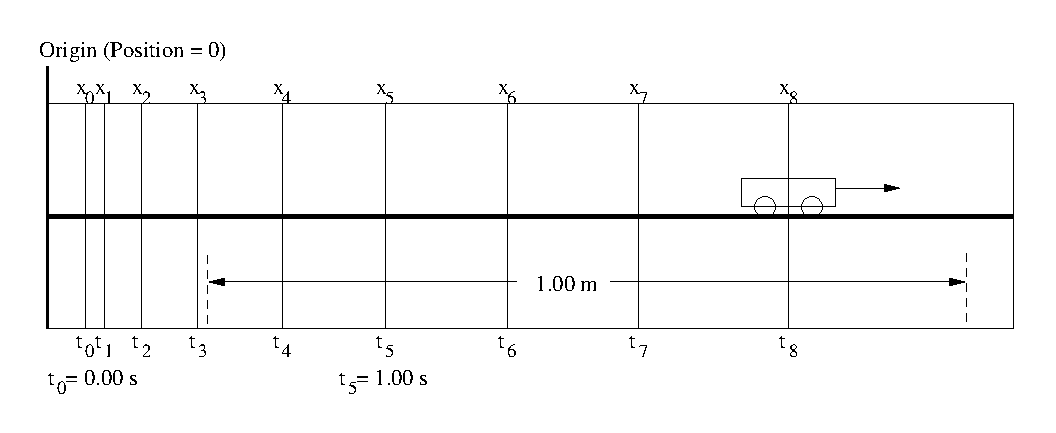
\includegraphics[trim={0.2cm 0 0.2cm 0},clip]{equations/equations_fig1.eps} \par}
\vspace{0.3cm}

\pagebreak[2]
\textbf{Activity 1: Position \textit{vs.}~Time from a Cart Video} 

(a) Let's start the measuring process by recording the key scaling factors that
will be used to calibrate the time and distance measurements. How much time,
t, has elapsed between frame 0 and frame 1, between frame 1 and frame 2, etc.
What is the calibration factor (i.e., how many real meters are represented by
each centimeter in the diagram)?

t =   \rule{1.0in}{0.1pt} s \hfill{}m/cm = \rule{1.0in}{0.1pt}

(b) Use a ruler to measure the cart's distance from the origin (i.e., its position)
in cm at each of the times (0.00 s, 0.20 s, etc.) and fill in columns 1 and
2 in table the below.

(c) Use the scaling factor between ``diagram centimeters'' and
real meters to calculate the position in meters of the cart. Place the results
in column 3.

\vspace{0.3cm}
{\centering \begin{tabular}{|c|c|c|c|c|c|}
\hline 
&
Distance from&
Elapsed &
Actual distance&
Average&
Average\\
&
origin in diagram&
time&
from origin&
velocity&
acceleration\\
&
1&
2&
3&
4&
5\\
Position&
$x$ (cm)&
$t$ (s)&
$x$ (m)&
$\langle v\rangle$ (m/s)&
$\langle a\rangle$ [(m/s)/s]\\
\hline 
\hline 
\( x_{0} \)&
&
0.000&
&
-&
-\\
\hline 
&
-&
0.100&
-&
&
-\\
\hline 
x\( _{1} \)&
&
0.200&
&
-&
\\
\hline 
&
-&
0.300&
-&
&
-\\
\hline 
\( x_{2} \)&
&
0.400&
&
-&
\\
\hline 
&
-&
0.500&
-&
&
-\\
\hline 
\( x_{3} \)&
&
0.600&
&
-&
\\
\hline 
&
-&
0.700&
-&
&
-\\
\hline 
\( x_{4} \)&
&
0.800&
&
-&
\\
\hline 
&
-&
0.900&
-&
&
-\\
\hline 
\( x_{5} \)&
&
1.000&
&
-&
\\
\hline 
&
-&
1.100&
-&
&
-\\
\hline 
\( x_{6} \)&
&
1.200&
&
-&
\\
\hline 
&
-&
1.300&
-&
&
-\\
\hline 
\( x_{7} \)&
&
1.400&
&
-&
\\
\hline 
&
-&
1.500&
-&
&
-\\
\hline 
\( x_{8} \)&
&
1.600&
&
-&
-\\
\hline 
\end{tabular}\par}
\vspace{0.3cm}

\textbf{How Do You Define Average Velocity Mathematically?}

By considering the work you did with the motion detector and with the measurements
you just performed in Activity 1, you should be able to define average velocity
along a line in words or even mathematically. Remember that velocity is the
rate of change of position divided by the time interval over which the change
occurred. 

Note: Mathematically, change is defined as the difference between the final
value of something minus the initial value of something.

{\par\centering Change = (Final Value) $-$ (Initial Value)\par}

\textbf{Activity 2: Defining Velocity in One Dimension} 

(a) Describe in words as accurately as possible what the word ``velocity''
means by drawing on your experience with studying velocity graphs of motion.
Hint: How can you tell from the graph the direction an object moves? How can
you tell how fast it is moving?
\answerspace{20mm}

\pagebreak[2]
(b) Suppose that you have a long tape measure and a timer to keep track of a
cart or your partner who is moving irregularly along a line. For the purposes
of this analysis, assume that the object of interest is a mere point mass. Describe
what you would need to measure and how you would use these measurements to calculate
velocity at a given moment in time.
\answerspace{20mm}

(c) Can you put this description in mathematical terms? Denote the
average velocity with the symbol $\langle v\rangle$. Suppose the
distance from the origin (where the motion detector was when it was
being used) to your partner is \( x_{1} \) at a time \( t_{1} \) just
before the moment of interest and that the distance changes to \(
x_{2} \) at a later time \( t_{2} \) which is just after the moment of
interest. Write the equation you would use to calculate the average
velocity, $\langle v\rangle$ , as a function of \( x_{1} \), \( x_{2} \), 
\( t_{1}
\), and \( t_{2} \).  What happens to the sign of $\langle v\rangle$
when \( x_{1}
\) is greater than \( x_{2} \)?
\answerspace{20mm}

(d) Use the mathematical definition in part (c) to calculate the average velocity
for each time interval of the cart motion described in Activity 1 and fill in
column 4 of the table in Activity 1. Show at least one sample calculation in
the space below. Important note: \( t_{2}  - t_{1} \) represents a time
interval, \( \Delta  t\), between two measurements of position and is not necessarily
the total time that has elapsed since a clock started.
\vspace{20mm}

\textbf{Defining Average Acceleration Mathematically} 

By considering the work you did with the motion detector, you should be able
to define average acceleration in one dimension mathematically. It is similar
to the mathematical definition of average velocity which you developed in Activity
2. All of the circumstances in which accelerations are positive and negative
are described by the equation that defines them. 

\textbf{Activity 3: Defining Average Acceleration }

(a) Describe in words as accurately as possible what the word ``acceleration''
means by drawing on your experience with studying velocity and acceleration
graphs of motion.
\answerspace{20mm}

(b) Suppose the cart's average velocity is $\langle v_{1}\rangle$
at a time \( t_{1} \)
and that the average velocity changes to $\langle v_2\rangle$
at a later time \( t_{2} \).
Write an equation for the average acceleration in the space below. 
\answerspace{20mm}

\pagebreak[2]
(c) Use the mathematical definition in part (b) to calculate the average acceleration
of the cart motion depicted in Activity 1 and fill in column 5 of the table
in Activity 1 for each time interval (i.e., 0.00 to 0.20 s, 0.20 s to 0.40 s,
etc.). Show at least one sample calculation in the space below.
\answerspace{20mm}

(d) Suppose you are walking away from a motion detector. How does the rate of
your walking change if $\langle v_{1}\rangle$ is greater than 
$\langle v_{2}\rangle$? Is your
acceleration positive or negative? Use the mathematical equation in part (b)
to explain your answer. 
\vspace{20mm}

(e) Suppose you are walking toward a motion detector. How is your speed (i.e.,
magnitude of velocity) changing for 
$\langle v_{1}\rangle > \langle v_{2} \rangle$? Is your
acceleration positive or negative? Be very careful with your mathematics on
this one. It's tricky!
\vspace{20mm}

(f) Is the sign of $\langle a\rangle$
always the same as the sign of the velocities? Why or
why not?
\vspace{20mm}

\textbf{Instantaneous Velocity and the Slope of a Position \textit{vs.}~Time Graph} 

What happens if we want to know the velocity of an object at a single instant?
That is, we'd like to estimate the velocity of an object during a time interval
which is too small to measure directly. Since velocity is a measure of the change
in position over time, it is possible to use techniques developed in calculus
to estimate how a continuously varying function of position \textit{vs.}~time changes
during a very short time interval. Let's start by considering how we might determine
the slope of a continuous function and proceed from there.

\textbf{Activity 4: Defining the Slope or Tangent} 

(a) In the figure below, what is the equation for the average slope of the curve
at the highlighted point in terms of \( x_{1} \), \( x_{2} \), \( t_{1} \),
and \( t_{2} \)?

%\vspace{0.3cm}
%{\par\raggedright 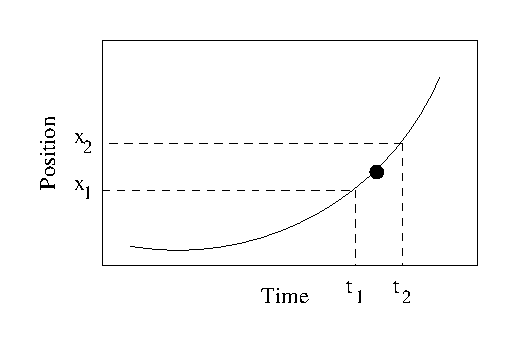
\includegraphics{equations/equations_fig2.eps} \par}
%\vspace{0.3cm}
\begin{lab_axis}[lab_noticks_1quad,
	width=2.0in,  height=1.5in,
	xlabel=Time,
	ylabel=Position,
	xtick={0.7,0.8},
	xticklabels={$t_1$,$t_2$},
	ytick={0.575,0.74},
	yticklabels={$x_1$,$x_2$},
	tick label style = {font=\itshape},
]
\addplot {1.5*(x-0.2)^2+0.2};
\addplot +[dashed,thick] coordinates {(0.7,0.0) (0.7,0.575) (0,0.575)};
\addplot +[dashed,thick] coordinates {(0.8,0.0) (0.8,0.74) (0,0.74)};
\end{lab_axis}

(b) How is the value of the slope related to the average velocity in the time
interval 
$[t_1,t_2]$?
\vspace{10mm}

(c) Since the rate of change of position is increasing as time goes on (so that
the position ``curve'' is not linear), how can you calculate
a more accurate value of the slope? Hint: Feel free to use different $x$ and 
$t$
values in your ``calculation'' to correspond to a different
time interval.
\vspace{20mm}

(d) How would you find the ``exact'' value of the slope at the
point in time of interest?
\vspace{20mm}

(e) Look up the formal definition of a derivative in your calculus book and
list it below. Usually it has to do with $f(x)$ and how it changes with $x$.
\vspace{20mm}

(f) Notice that in our position \textit{vs.}~time graph we are interested in how $x$ 
changes
with $t$. Thus, we would use the notation $x(t)$ to indicate that 
$x$ is a function
of $t$. By letting $x$ play the role of $f$ and $t$ play the role of 
$x$, rewrite the
definition of the derivative.
\vspace{20mm}

(g) How might the instantaneous value of velocity at the highlighted point be
related to the derivative of $x$ with respect to $t$ at that same point?
\vspace{20mm}

(h) Suppose that $x(t) = t^{2} + 1$, where $x$ is in centimeters and $t$ is
in seconds. What is the derivative of this function with respect to time? What
is its instantaneous velocity?
\vspace{20mm}

(i) What is the instantaneous velocity, $v$, in cm/s at $t = 1$ s? At 
$t = 2$ s?
\answerspace{20mm}

\pagebreak[2]
\textbf{Acceleration as the Slope of a Velocity Graph} 

Just as velocity is the rate of change of position, acceleration is the rate
of change of velocity. How do we find the acceleration of an object at a single
instant (i.e., during a time interval which is too small to measure directly).
Since acceleration is the rate of change of velocity, the acceleration of an
object is given by the slope of a smooth curve drawn through its velocity vs.
time graph.

Let's apply this graphical analysis approach to the task of finding the instantaneous
acceleration for the cart motion described in Activity 1.

\textbf{Activity 5: Accelerations from the Cart Data }

(a) Refer to the data that you analyzed and recorded in the table in Activity
1. Use Excel to fit the velocity ($y$ axis) \textit{vs.}~time ($x$ axis) data with
a line. Label the resulting graph and put a copy in your notebook. The slope
of the line represents the acceleration of the cart. Report its value in the
space below.
\vspace{10mm}

(b) How does the value for acceleration which you determined from the slope
compare to those you determined earlier from the average accelerations at the
mid-point of each time interval between average velocity values. In other words,
how does the slope compare with the averages reported in column 5 of the table
in Activity 1? Find the average and standard deviation of the elements in column
5 of the table and report them in the space below. (You can use Excel
for this.)
\vspace{20mm}

(c) Does the acceleration determined by the slope lie within one standard deviation
of the average of the average accelerations? 

